\begin{center}\textbf{\color{red}LUYỆN TẬP}\\
	\textbf{Bài 5. CHUYỂN ĐỘNG TỔNG HỢP}
\end{center}
\section{TRẮC NGHIỆM}
\Opensolutionfile{ans}[ans/BAI5-TN]
% ===================================================================
\begin{ex}
Một người đi xe máy từ nhà đến bến xe bus cách nhà $\SI{6}{\kilo\meter}$ về phía Đông. Người đó tiếp tục lên xe bus đi tiếp $\SI{6}{\kilo\meter}$ về phía Bắc. Độ dịch chuyển tổng hợp của người này là	
	\choice
	{$\SI{12}{\kilo\meter}$}
	{$\SI{6}{\kilo\meter}$}
	{\True $\xsi{6\sqrt{2}}{\kilo\meter}$}
	{$\SI{72}{\kilo\meter}$}
	\loigiai{}
\end{ex}
% ===================================================================
\begin{ex}
	Gọi $\vec{v}_{12}$ là vận tốc của vật (1) so với vật (2), $\vec{v}_{23}$ là vận tốc của vật (2) so với vật (3), $\vec{v}_{13}$ là vận tốc của vật (1) so với vật (3). Hệ thức đúng là
	\choice
	{$\vec{v}_{13}=\vec{v}_{12}-\vec{v}_{23}$}
	{$\vec{v}_{13}=\vec{v}_{12}+2\vec{v}_{23}$}
	{\True $\vec{v}_{13}=\vec{v}_{12}+\vec{v}_{23}$}
	{$\vec{v}_{13}=2\vec{v}_{12}+\vec{v}_{23}$}
	\loigiai{}
\end{ex}
% ===================================================================
\begin{ex}
	Một hành khách ngồi trong xe A, nhìn qua cửa sổ thấy xe B bên cạnh và sân ga đều chuyển động như nhau. Như vậy
	\choice
	{xe A đứng yên, xe B chuyển động}
	{\True xe A chạy, xe B đứng yên}
	{xe A và xe B chạy cùng chiều}
	{xe A và xe B chạy ngược chiều}
	\loigiai{}
\end{ex}
% ===================================================================
\begin{ex}
Hai ô tô A và B chạy cùng chiều trên cùng một đoạn đường với tốc độ $\SI{70}{\kilo\meter/\hour}$ và $\SI{65}{\kilo\meter/\hour}$. Tốc độ của ô tô A so với ô tô B bằng	
	\choice
	{$\SI{30}{\kilo\meter/\hour}$}
	{\True $\SI{5}{\kilo\meter/\hour}$}
	{$\SI{135}{\kilo\meter/\hour}$}
	{$\SI{65}{\kilo\meter/\hour}$}
	\loigiai{}
\end{ex}
% ===================================================================
\begin{ex}
	A ngồi trên một toa tàu chuyển động với tốc độ $\SI{15}{\kilo\meter/\hour}$ đang rời ga. B ngồi trên một toa tàu khác chuyển động với tốc độ $\SI{10}{\kilo\meter/\hour}$ đang đi ngược chiều vào ga. Hai đường tàu song song với nhau. Chọn chiều dương là chiều chuyển động của đoàn tàu mà A ngồi. Vận tốc của B đối với A là
	\choice
	{$\SI{-5}{\kilo\meter/\hour}$}
	{$\SI{5}{\kilo\meter/\hour}$}
	{$\SI{25}{\kilo\meter/\hour}$}
	{\True $\SI{-25}{\kilo\meter/\hour}$}
	\loigiai{}
\end{ex}
% ===================================================================
\begin{ex}
Hai bến sông A và B cùng nằm trên một bờ sông, cách nhau $\SI{18}{\kilo\meter}$. Cho biết độ lớn vận tốc của ca nô đối với nước là $u =\SI{16.2}{\kilo\meter/\hour}$ và độ lớn vận tốc của nước đối với bờ sông là $v=\SI{5.4}{\kilo\meter/\hour}$. Thời gian để ca nô chạy xuôi dòng từ A đến B rồi lại chạy ngược dòng trở về A là	
	\choice
	{1 giờ 40 phút}
	{1 giờ 20 phút}
	{\True 2 giờ 30 phút}
	{2 giờ 10 phút}
	\loigiai{}
\end{ex}
% ===================================================================
\begin{ex}
Ô tô A chạy thẳng về hướng Tây với độ lớn vận tốc $\SI{40}{\kilo\meter/\hour}$. Ô tô B chạy thẳng về hướng Bắc với độ lớn vận tốc $\SI{60}{\kilo\meter/\hour}$. Độ lớn vận tốc của ô tô B so với người ngồi trên ô tô A gần giá trị nào nhất sau đây?	
	\choice
	{$\SI{85}{\kilo\meter/\hour}$}
	{$\SI{90}{\kilo\meter/\hour}$}
	{$\SI{65}{\kilo\meter/\hour}$}
	{\True $\SI{75}{\kilo\meter/\hour}$}
	\loigiai{}
\end{ex}
% ===================================================================
\begin{ex}
	Một chiếc xuồng đi xuôi dòng nước từ A đến B mất 4 giờ, còn nếu đi ngược dòng nước từ B đến A mất 5 giờ. Biết vận tốc của dòng nước so với bờ sông là $\SI{4}{\kilo\meter/\hour}$. Quãng đường AB là
	\choice
	{\True $\SI{160}{\kilo\meter}$}
	{$\SI{120}{\kilo\meter}$}
	{$\SI{130}{\kilo\meter}$}
	{$\SI{150}{\kilo\meter}$}
	\loigiai{}
\end{ex}
% ===================================================================
\begin{ex}
	Một người lái xuồng máy cho xuồng chạy ngang con sông rộng $\SI{240}{\meter}$. Mũi xuồng luôn luôn vuông góc với bờ sông, nhưng do nước chảy nên xuồng sang đến bờ bên kia tại một điểm cách bến dự định $\SI{180}{\meter}$ về phía hạ lưu và xuồng đi hết 1 phút. Độ lớn vận tốc của xuồng so với bờ là
	\choice
	{$\SI{8}{\meter/\second}$}
	{$\SI{9}{\meter/\second}$}
	{$\SI{6}{\meter/\second}$}
	{\True $\SI{5}{\meter/\second}$}
	\loigiai{}
\end{ex}
% ===================================================================
\begin{ex}
	Nhà của Bách và trường nằm trên cùng một con đường nên hằng ngày Bách đều đi học bằng xe đạp từ nhà đến trường với tốc độ không đổi bằng $\SI{4}{\meter/\second}$ (khi trời lặng gió). Trong một lần Bách đạp xe từ nhà đến trường, có một cơn gió thổi ngược chiều trong khoảng thời gian $\SI{90}{\second}$ . Hình bên mô tả đồ thị độ dịch chuyển - thời gian của Bách trong 5 phút đầu tiên. Tốc độ của gió so với mặt đất là bao nhiêu?
\begin{center}
		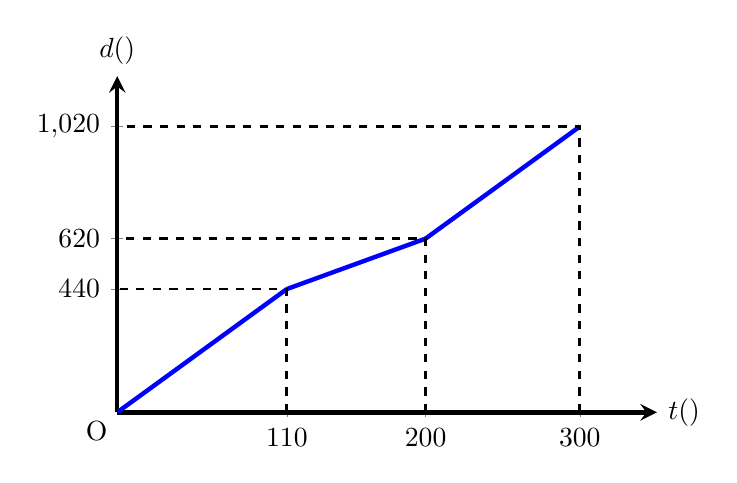
\begin{tikzpicture}  
		\begin{axis}[  ultra thick,yscale=0.75,
			xmin=0,  
			xmax=350,  
			xtick={0,110,200,300},
			ytick={0,440,620,1020},
			minor x tick num=0,
			minor y tick num=0,
			ymin=0,  
			ymax=1200, 
			samples=300,
			axis lines=center, 
			xlabel=$\xsi{t}{\left(\si{\second}\right)}$, 		ylabel=$\xsi{d}{\left(\si{\meter}\right)}$,
			every axis y label/.style={at=(current axis.above origin),anchor=south},  
			every axis x label/.style={at=(current axis.right of origin),anchor=west},  ]
			\addplot [ultra thick, blue, smooth, domain=0:110] {4*x};  
			\addplot [ultra thick, blue, smooth, domain=110:200] {440+2*(x-110)}; 
			\addplot [ultra thick, blue, smooth, domain=200:300] {620+4*(x-200)}; 
			\draw[dashed, line width=1pt] (axis cs: 110,0)--(axis cs:110,440)--(axis cs:0,440);
			\draw[dashed, line width=1pt] (axis cs: 200,0)--(axis cs:200,620)--(axis cs:0,620);
			\draw[dashed, line width=1pt] (axis cs: 300,0)--(axis cs:300,1020)--(axis cs:0,1020);
		\end{axis}  
		\node[below left] at(0,0) {O};
	\end{tikzpicture}
\end{center}
	\choice
	{$\SI{1.2}{\meter/\second}$}
	{$\SI{1.5}{\meter/\second}$}
	{\True $\SI{2}{\meter/\second}$}
	{$\SI{2.5}{\meter/\second}$}
	\loigiai{}
\end{ex}

\Closesolutionfile{ans}
\section{TỰ LUẬN}
\setcounter{ex}{0}
% ======================================================================
\begin{ex}
Một ca nô chạy hết tốc lực trên mặt nước yên lặng có thể đạt $\SI{21,5}{km/h}$. Ca nô này chạy xuôi dòng sông trong 1 giờ rồi quay lại thì phải mất 2 giờ nữa mới về tới vị trí ban đầu. Hãy tính tốc độ của dòng nước.	
	\loigiai{$\SI{7.17}{\kilo\meter/\hour}$}
\end{ex}
% ======================================================================
\begin{ex}
	Một máy bay đang bay theo hướng Bắc với vận tốc $\SI{200}{m/s}$ thì bị gió từ hướng Tây thổi vào với vận tốc $\SI{20}{m/s}$. Xác định vận tốc tổng hợp của máy bay lúc này.
	\loigiai{}
\end{ex}
% ======================================================================
\begin{ex}
	Một người lái tàu vận chuyển hàng hoá xuôi dòng từ sông Đồng Nai đến khu vực cảng Sài Gòn với tốc độ là $\SI{40}{\kilo\meter/\hour}$ so với bờ. Sau khi hoàn thành công việc, lái tàu quay lại sông Đồng Nai theo lộ trình cũ với tốc độ là $\SI{30}{\kilo\meter/\hour}$ so với bờ. Biết rằng chiều và tốc độ của dòng nước đối với bờ không thay đổi trong suốt quá trình tàu di chuyển, ngoài ra tốc độ của tàu so với nước cũng được xem là không đổi. Hãy xác định tốc độ của dòng nước so với bờ.
	\loigiai{$\SI{5}{\kilo\meter/\hour}$}
\end{ex}
% ======================================================================
\begin{ex}
	Một người chèo thuyền qua một con sông rộng $\SI{400}{\meter}$. Muốn cho thuyền đi theo đường AB thì người đó phải luôn hướng mũi thuyền theo hướng AC. Biết thuyền qua sông hết $\SI{8}{\minute} \SI{20}{\second}$ và tốc độ của dòng nước là $\SI{0.6}{\meter/\second}$. Tìm tốc độ của thuyền so với dòng nước.
	\begin{center}
		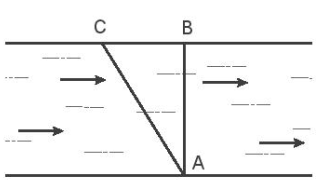
\includegraphics[width=0.35\linewidth]{figs/BAI5-1}
	\end{center}
	\loigiai{$\SI{1}{\meter/\second}$.}
\end{ex}
% ======================================================================
\begin{ex}
	Tại một thời điểm, ở vị trí M trên đoạn đường thẳng có xe máy A chạy qua với tốc độ $\SI{30}{\kilo\meter/\hour}$. Sau 10 phút, cũng tại vị trí M , có xe máy B chạy qua với tốc độ $\SI{40}{\kilo\meter/\hour}$ để đuổi theo xe máy A . Giả sử hai xe máy chuyển động thẳng với tốc độ xem như không đổi.
	\begin{enumerate}[label=\alph*)]
		\item Tính thời gian để xe máy B đuổi kịp xe máy A.
		\item Tính quãng đường mà xe máy A đã đi được đến khi xe máy B đuổi kịp.
	\end{enumerate}
	\loigiai{
	\begin{enumerate}[label=\alph*)]
		\item $\SI{0.5}{\hour}$.
		\item $\SI{15}{\kilo\meter}$.
	\end{enumerate}
	}
\end{ex}
% ======================================================================
\begin{ex}
	Một ô tô đang chạy với vận tốc $v$ theo phương nằm ngang thì người ngồi trong xe trông thấy giọt mưa rơi tạo thành những vạch làm với phương thẳng đứng một góc $\SI{45}{\degree}$. Biết vận tốc rơi của các giọt nước mưa so với mặt đất là $\SI{5}{\meter/\second}$. Tính vận tốc của ô tô.
	\loigiai{$\SI{5}{\meter/\second}$}
\end{ex}
% ======================================================================
\begin{ex}
	Một ca nô chạy ngang qua một dòng sông, xuất phát từ A , hướng mũi về B . Sau $\SI{100}{\second}$, ca nô cập bờ bên kia ở điểm C cách B $\SI{200}{\meter}$. Nếu người lái hướng mũi ca nô theo hướng AD và vẫn giữ tốc độ máy như cũ thì ca nô sẽ cập bờ bên kia tại đúng điểm B. Tìm:
	\begin{center}
		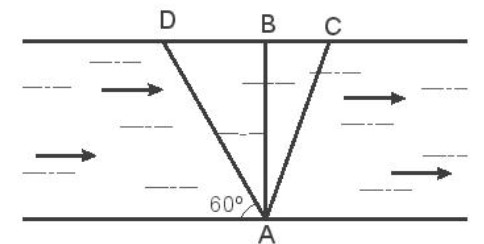
\includegraphics[width=0.35\linewidth]{figs/BAI5-2}
	\end{center}
	\begin{enumerate}[label=\alph*)]
		\item Vận tốc của dòng nước so với bờ sông.
		\item Vận tốc của ca nô so với dòng nước.
		\item Chiều rộng của sông.
	\end{enumerate}
	\loigiai{
	\begin{enumerate}[label=\alph*)]
		\item $\SI{2}{\meter/\second}$.
		\item $\SI{4}{\meter/\second}$.
		\item $\SI{400}{\meter}$.
	\end{enumerate}
	}
\end{ex}
% ======================================================================
\begin{ex}
	Hai xe chuyển động trên hai đường vuông góc với nhau, xe A đi về hướng tây với tốc độ $\SI{50}{\kilo\meter/\hour}$, xe B đi về hướng Nam với tốc độ $\SI{30}{\kilo\meter/\hour}$. Vào một thời điểm nào đó xe A và B còn cách giao điểm của hai đường lần lượt là $\SI{4.4}{\kilo\meter}$ và $\SI{4}{\kilo\meter}$, hai xe đang tiến về phía giao điểm. Tìm khoảng cách ngắn nhất giữa hai xe.\\
	\textit{(Hãy tính bài này bằng 2 cách: dùng phương pháp tọa độ và dùng vận tốc tương đối!!!)}
	\loigiai{
		$\SI{1.166}{\kilo\meter}$.
	}
\end{ex}
\begin{center}
	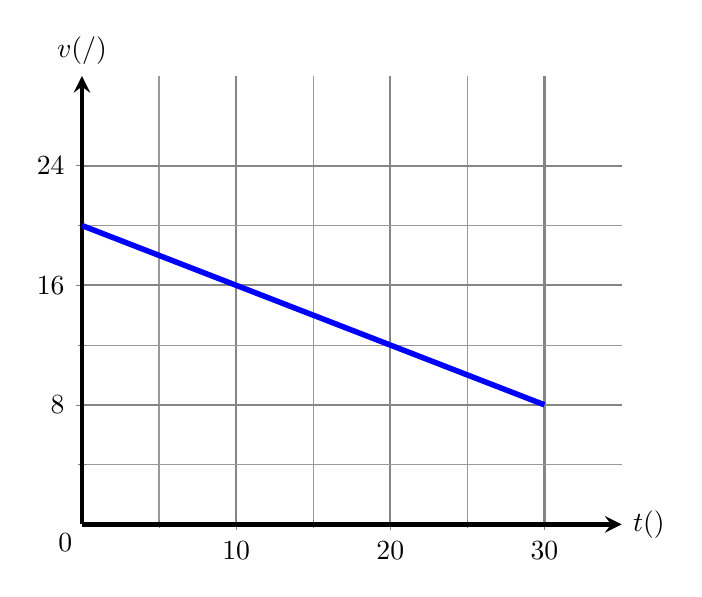
\begin{tikzpicture}  
		\begin{axis}[  ultra thick,
			xmin=0,  
			xmax=35,  
			xtick={0,10,...,30},
			ytick={0,8,...,24},
			minor x tick num=1,
			minor y tick num=1,
			ymin=0,  
			ymax=30, 
			samples=300,
			axis lines=center, 
			grid style={step=1, line width =0.4pt, color=gray!80!white},
			grid=both, %giới hạn ô lưới
			major grid style={line width=0.8pt,gray!95!white},
			xlabel=$\xsi{t}{\left(\si{\second}\right)}$, 		ylabel=$\xsi{v}{\left(\si{\meter/\second}\right)}$,
			every axis y label/.style={at=(current axis.above origin),anchor=south},  
			every axis x label/.style={at=(current axis.right of origin),anchor=west},  ]
			\addplot [line width=2pt, blue, smooth, domain=0:30] {20-0.4*x};  
			\coordinate (O) at (0,0);
		\end{axis}  
		\node[below left] at (O) {0};
	\end{tikzpicture}
\end{center}
\begin{center}
	\textbf{--- HẾT ---}
\end{center}